%\documentclass[Serif, 10pt, brown, handout]{beamer} % Disable overlays for handout format
%\documentclass[Serif, 10pt, brown, handout, notes]{beamer} % Disable overlays for handout format and print notes
\documentclass[Serif, 10pt, brown]{beamer}
\usepackage{booktabs,xcolor}
%\usepackage[svgnames,table]{xcolor}
%\usepackage[tableposition=above]{caption}
\usepackage{pifont}
\newcommand*\CHECK{\ding{51}}
\usepackage{array}
\newcolumntype{P}[1]{>{\centering\arraybackslash}p{#1}}
%
\usepackage{setspace,mathtools,amssymb,multirow,array,amsmath,tikz}
\usepackage[normalsize]{subfigure}
\usetikzlibrary{patterns}
\usetikzlibrary{automata,positioning,decorations.pathreplacing,decorations}

\usepackage{curves}
\usepackage{wasysym}
\usepackage{epsfig,epstopdf,graphicx}

\curvewarnfalse
%
\newtheorem{proposition}{Proposition}
\theoremstyle{example}
\newtheorem{theoremh}{Theorem}
\theoremstyle{plain}
\renewcommand{\textfraction}{0.01}
\renewcommand{\floatpagefraction}{0.99}
\newcommand{\ul}{\underline}
\newcounter{units}
%
\usepackage[round]{natbib}
 \bibpunct[, ]{(}{)}{,}{a}{}{,}%
 \def\bibfont{\small}%
 \def\bibsep{\smallskipamount}%
 \def\bibhang{24pt}%
 \def\newblock{\ }%
 \def\BIBand{and}%
%
\setbeamercovered{dynamic}
% Logo
%\logo{\includegraphics[width=0.in,keepaspectratio]{logo.jpg}}
%
% Setup
\mode<presentation>
	{
\usetheme[right,currentsection, hideothersubsections]{UTD}
			\useoutertheme{sidebar} \useinnertheme[shadow]{rounded}
			\usecolortheme{whale} \usecolortheme{orchid}
			\usefonttheme[onlymath]{serif}
			\setbeamertemplate{footline}{\centerline{Slide \insertframenumber/\inserttotalframenumber}}
	}
%
% Title
\usebeamercolor[fg]{author in sidebar}
\title[{Paper Short Title}]{\sc Gate Level Minimization}
\author[\ul{Authors}]{{\bf Authors}\\ \scriptsize{(Joint work of {\bf Group13})}}
\institute[UTD]{\sc\small Indian Institute Of Technology Hyderabad}%\\ \sf \small Naveen Jindal School of Management}
\date[UCI]{Digital Systems \\ Date 2024}
%
%Presentation
\begin{document}
\frame{\titlepage}
%
%
%Slides

%TOC

\begin{frame}
	\transblindsvertical
	\frametitle{Contents}
	\tableofcontents[hidesubsections]
\end{frame}
\note[itemize]{
\item Here's the overall structure of my talk today.
}


% Introduction
\section[Introduction]{Introduction}

\setbeamercolor{background canvas}{use=structure,bg=white}
\setbeamercolor{background}{use=structure,bg=white}
\begin{frame}{Introduction}
    \begin{itemize}
\item  \textbf{Gate-level minimization} is the design task of finding an optimal gate-level implementation
of the Boolean functions describing a digital circuit.
\item It is too difficult to execute it by manual method when the logic has more number of inputs.
\item This problem has been solved by computer-based logic synthesis tools that minimize
a large set of Boolean equations efficiently and quickly.
\end{itemize}
\end{frame}



\section[Map Method]{Map Method}
\begin{frame}
	\frametitle{Map Method}
	\transfly
	\begin{itemize}
    \item The Map Method is the simple,straight forward procedure for minimizing Boolean functions Known as Karnaugh Maps(K-Maps)
        \item K-Maps are a visual representation of truth tables.
        \item Adjacent cells differ by one variable, enabling simplification.
        \item K-Maps exist for 2, 3, 4, and 5 variables.
    \end{itemize}
	\begin{exampleblock}{Note}
		The main assumption in the K-map method:\\
        \textbf{The simplest algebraic
expression is one that has a minimum number of terms with the smallest possible number
of literals in each term.}
	\end{exampleblock}

\end{frame}

\section[2 Variable K-Map]{2 Variable K-Map}
\begin{frame}
	\frametitle{2 Variable K-Map}
	\transfly
	\begin{itemize}
        \item Four squares representing minterms.
        
        \item Simplified expressions minimize gates and inputs.
        \begin{center}
        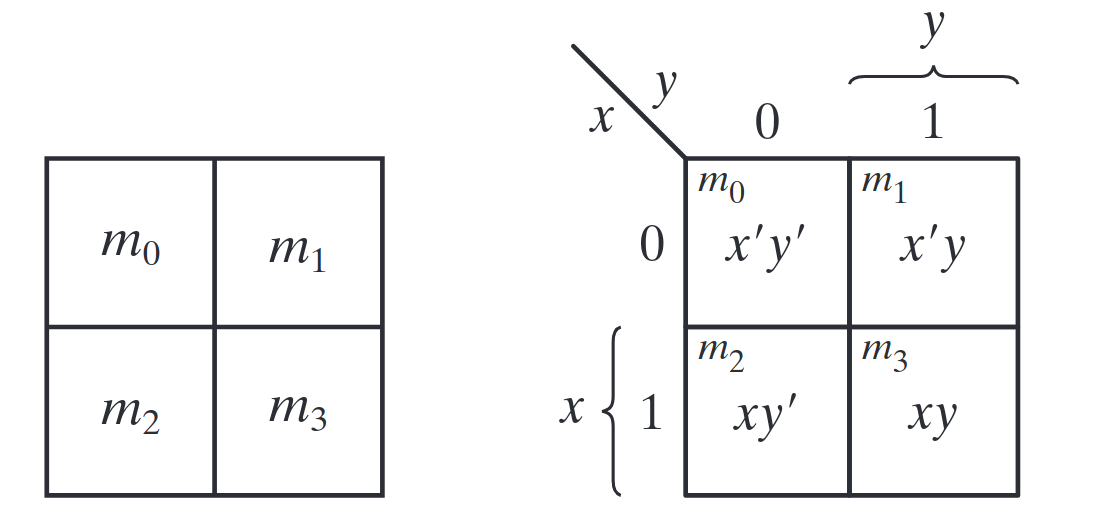
\includegraphics[width=0.5\linewidth]{figs/2var.png}
    \end{center}
    \item Example: \( F(x,y) = xy \)  and \( F(x,y) = x+y \)
    \begin{center}
        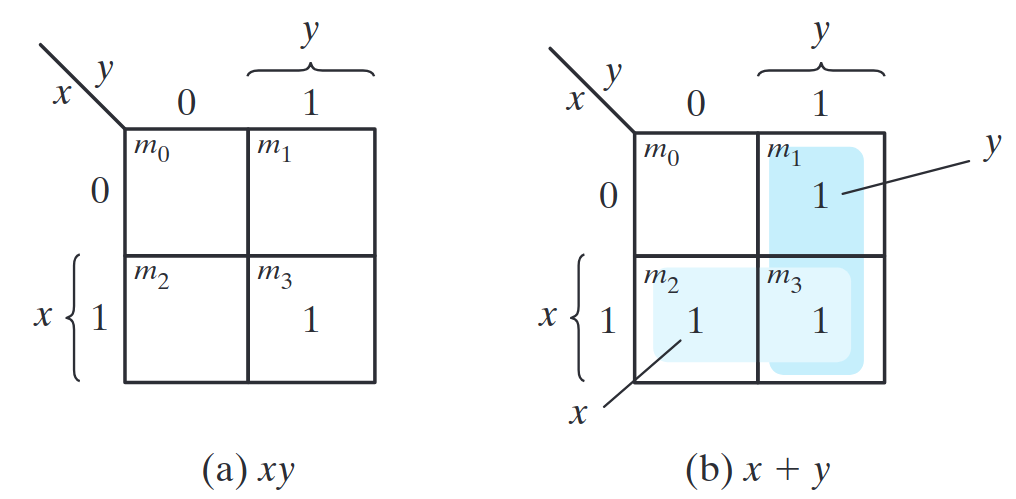
\includegraphics[width=0.5\linewidth]{figs/2ex.png}
    \end{center}
    \end{itemize}
    
	

\end{frame}
\section[3 Variable K-Map]{3 Variable K-Map }
\begin{frame}
	\frametitle{3 Variable K-Map }
	\transfly
	 \begin{itemize}
        \item 8 squares arranged in Gray code sequence.
        \item Adjacent squares differ by only one variable.
        
    
    \begin{center}
        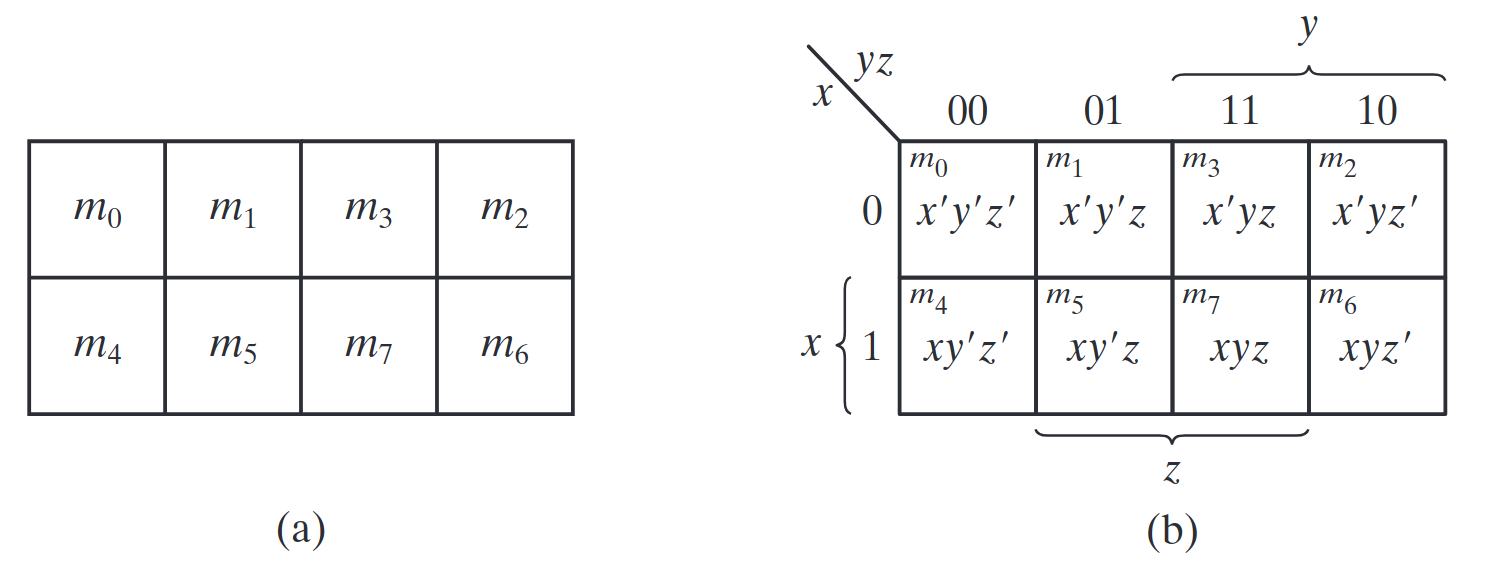
\includegraphics[width=0.6\linewidth]{figs/3var.png}
    \end{center}
    \item Example 1: \( F(x,y,z) = \Sigma(2,3,4,5) \rightarrow x' y + xy' \)
    \begin{center}
        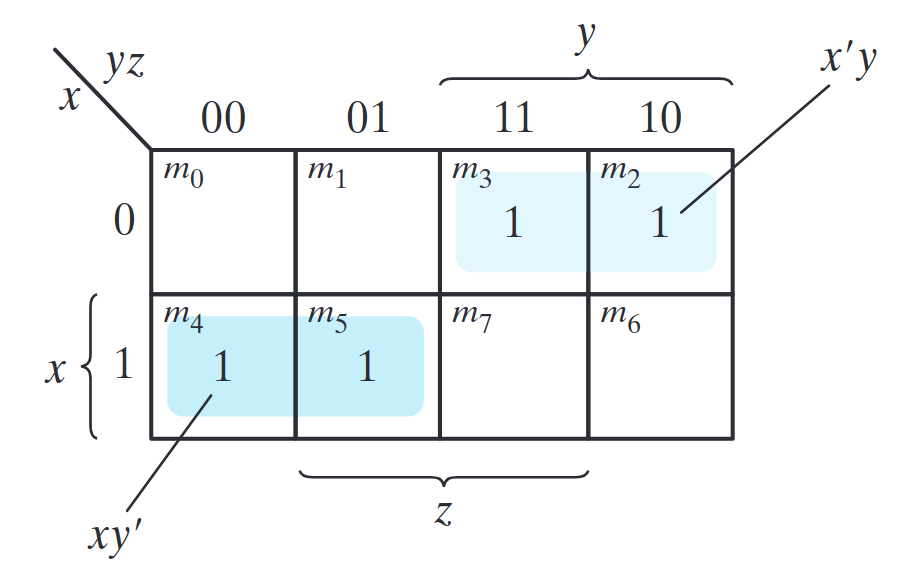
\includegraphics[width=0.5\linewidth]{figs/3ex1.png}
    \end{center}
    \end{itemize}
	

\end{frame}
%\section[3 Variable K-Map examples]{3 Variable K-Map examples}
\begin{frame}
	\frametitle{3 Variable K-Map examples}
	\transfly
	 \begin{itemize}
       \item Example 2: \( F(x,y,z) = \Sigma(3,4,6,7) \rightarrow yz + xz' \)
    \begin{center}
        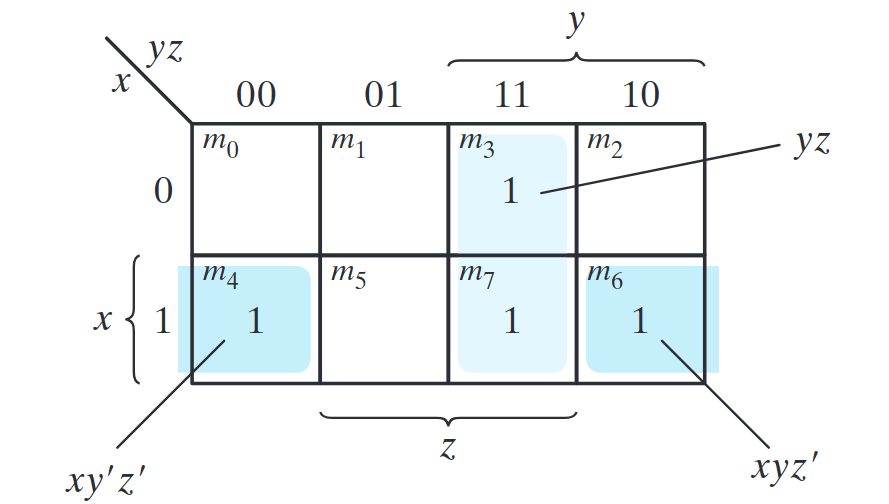
\includegraphics[width=0.5\linewidth]{figs/3ex2.png}
    \end{center}
    \item Example 3: \( F(x,y,z) = \Sigma(0,2,4,5,6) \rightarrow z' + xy' \)
    \begin{center}
        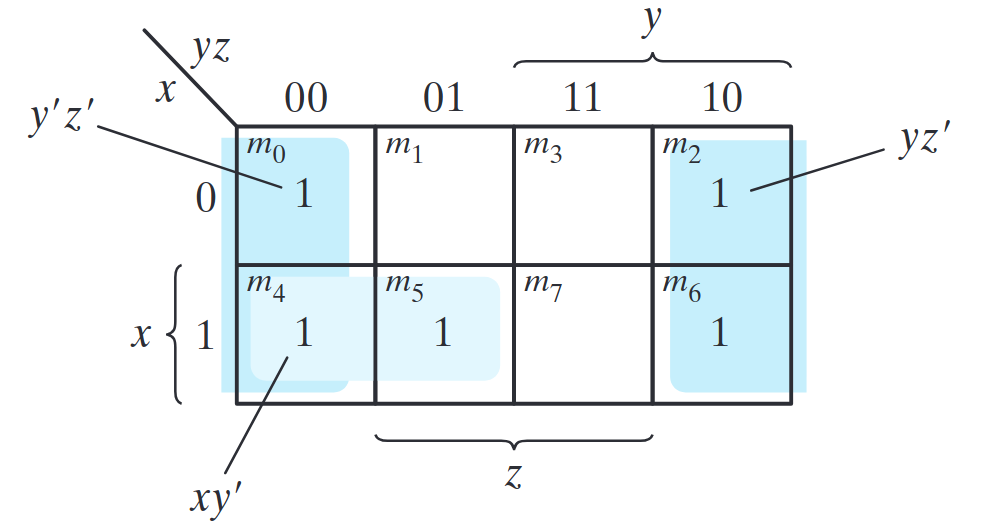
\includegraphics[width=0.5\linewidth]{figs/3ex3.png}
    \end{center}
    \end{itemize}
	

\end{frame}
\section[4 Variable K-Map]{4 Variable K-Map }
\begin{frame}
	\frametitle{4 Variable K-Map }
	\transfly
	 \begin{itemize}
        \item 16 squares, organized using Gray code.
        \item Allows simplifications of larger functions.
    
    \begin{center}
        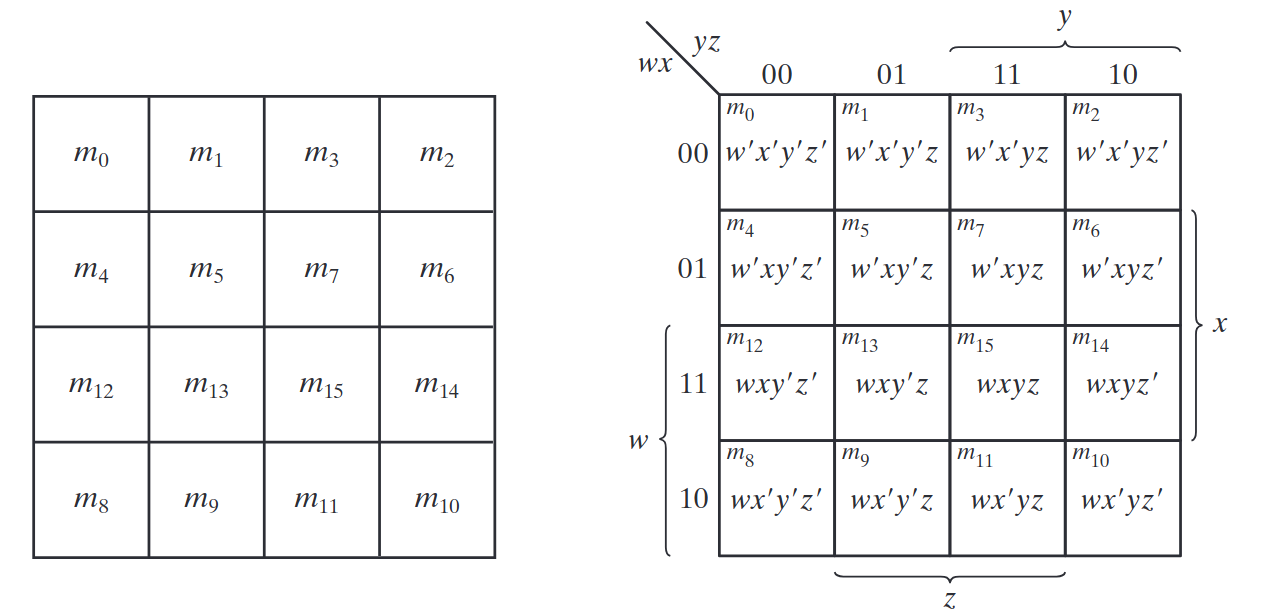
\includegraphics[width=0.625\linewidth]{figs/4var.png}
    \end{center}
    \item \( F(w,x,y,z) = \Sigma(0,1,2,4,5,6,8,9,12,13,14) \rightarrow y' + w' z' + x z' \)
    \begin{center}
        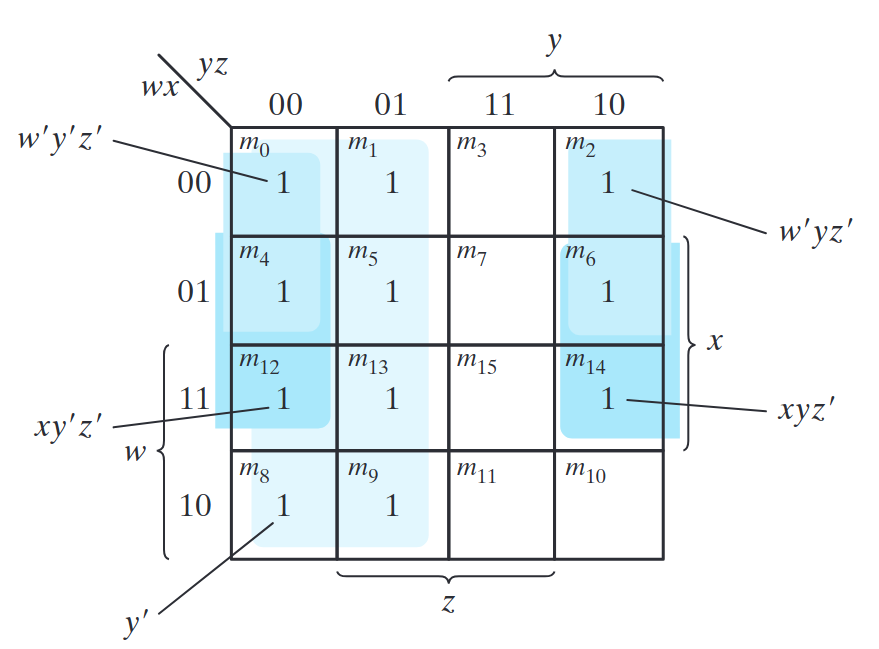
\includegraphics[width=0.5\linewidth]{figs/4ex.png}
    \end{center}
    \end{itemize}
\end{frame}

\section[Prime Implicants]{Prime Implicants}
\begin{frame}{Prime Implicants}
	\begin{itemize}
	    \item A \textbf{prime implicant} is a product term obtained by combining the maximum possible number of adjacent squares in a Karnaugh map (K-map). An implicant is \textbf{prime} if no other implicant with fewer literals covers it.
        \item A \textbf{prime implicant} is \textbf{essential} if a minterm is covered only by that implicant. Essential prime implicants \textbf{must} be included in the simplified function.
	\end{itemize}
    \begin{enumerate}
        \item Procedure for Finding Prime Implicants:
    
\begin{itemize}
    \item A single \textbf{1} in the K-map is a prime implicant if it has no adjacent 1s.
    \item Two adjacent \textbf{1s} form a prime implicant unless they are part of a larger group.
    \item Four adjacent \textbf{1s} form a prime implicant unless they are part of a group of eight.
\end{itemize}
\end{enumerate}
\end{frame}
\begin{frame}
	\frametitle{Example}
    \begin{itemize}
       \item Example: \( F(A,B,C,D) = \Sigma(0,2,3,5,7,8,9,10,11,13,15)\)
       \begin{center}
        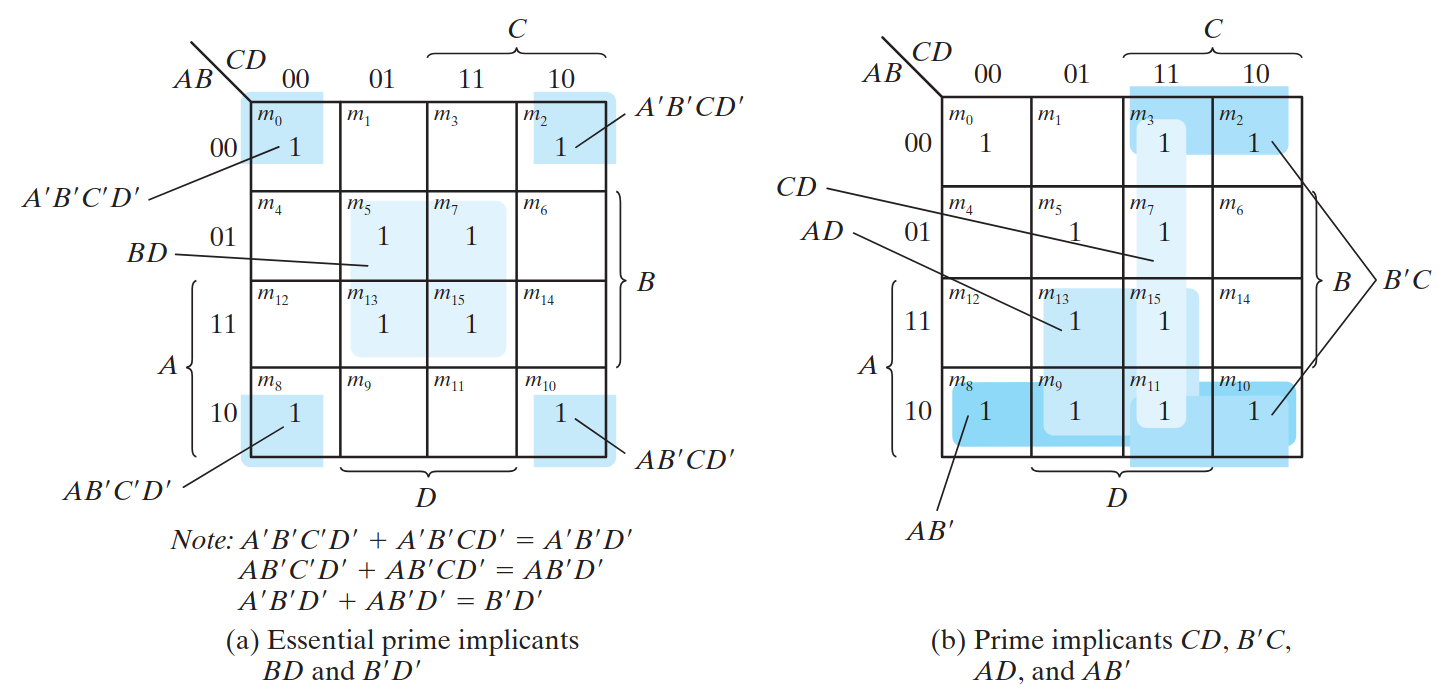
\includegraphics[width=0.5\textwidth]{figs/pr.png}
    \end{center}
    \item \( F  = BD + B'D + CD + AD\)
    \item \( F  = BD + B'D + CD + AB'\)
    \item \( F  = BD + B'D + B'C + AD\)
    \item \( F  = BD + B'D + B'C + AB'\)
    \end{itemize}
\end{frame}
\section[Product Of Sums]{Product Of Sums}
\begin{frame}{Sum-of-Products (SOP) and Product-of-Sums (POS)}
    \begin{itemize}
        \item SOP: OR-ing product terms (AND gates to OR gate).
        \item POS: AND-ing sum terms (OR gates to AND gate).
        \item Example: \( F(A,B,C,D) = \Sigma(0,1,2,5,8,9,10)\)\\\( F' = AB+CD+BD' \) (SOP), \( F = (A' + B') (C' + D' )(B'+D) \) (POS)
        \begin{center}
        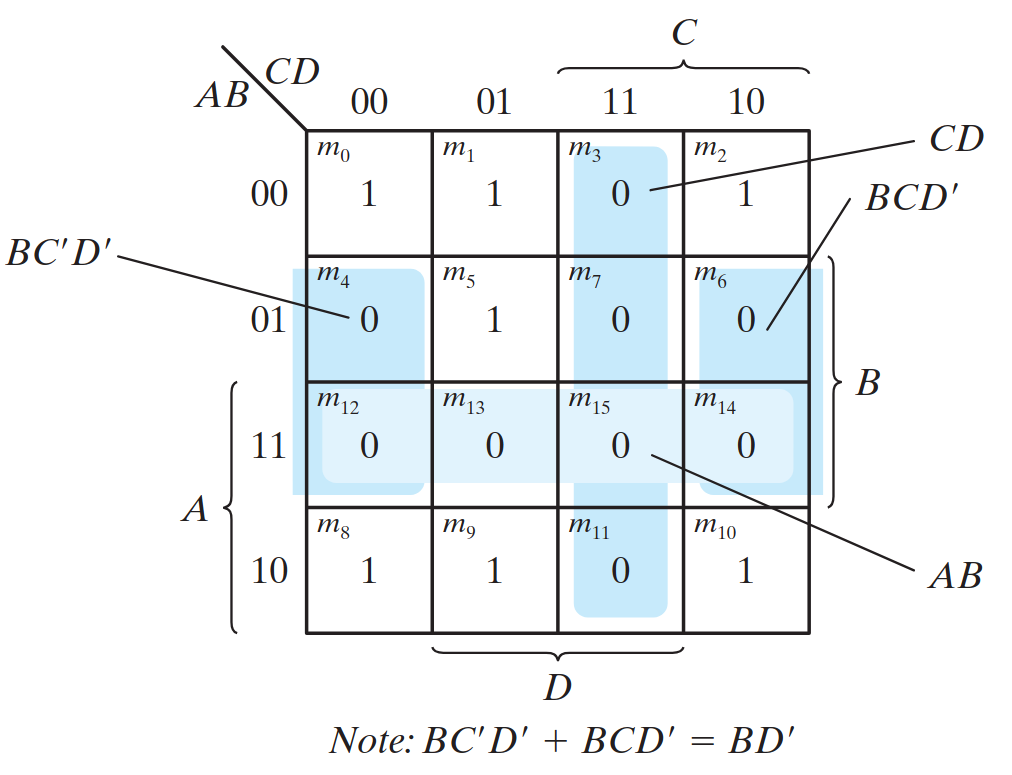
\includegraphics[width=0.5\textwidth]{figs/sop.png}
    \end{center}
    \end{itemize}
\end{frame}
\begin{frame}
    \begin{center}
        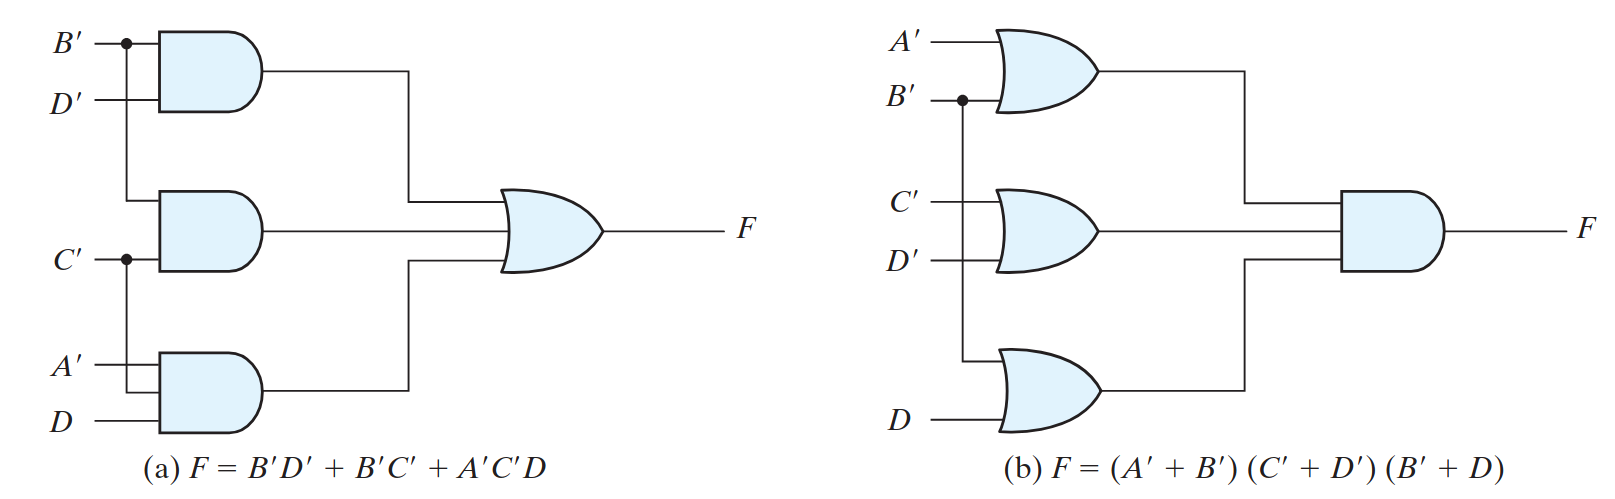
\includegraphics[width=\textwidth]{figs/gate.png}
    \end{center}
\end{frame}




\section[Don't Care Conditions]{Don't Care Conditions}
\begin{frame}{Don't Care Conditions}
    \begin{itemize}
        \item Unused input combinations can be treated as 0 or 1 for simplification.
        \item Helps minimize logic further.
        \item Example: \( F(w,x,y,z) = \Sigma(1,3,7,11,15) \) with don't-cares \( \Sigma(0,2,5) \) simplifies to \( yz + w'x' \)
        \begin{center}
        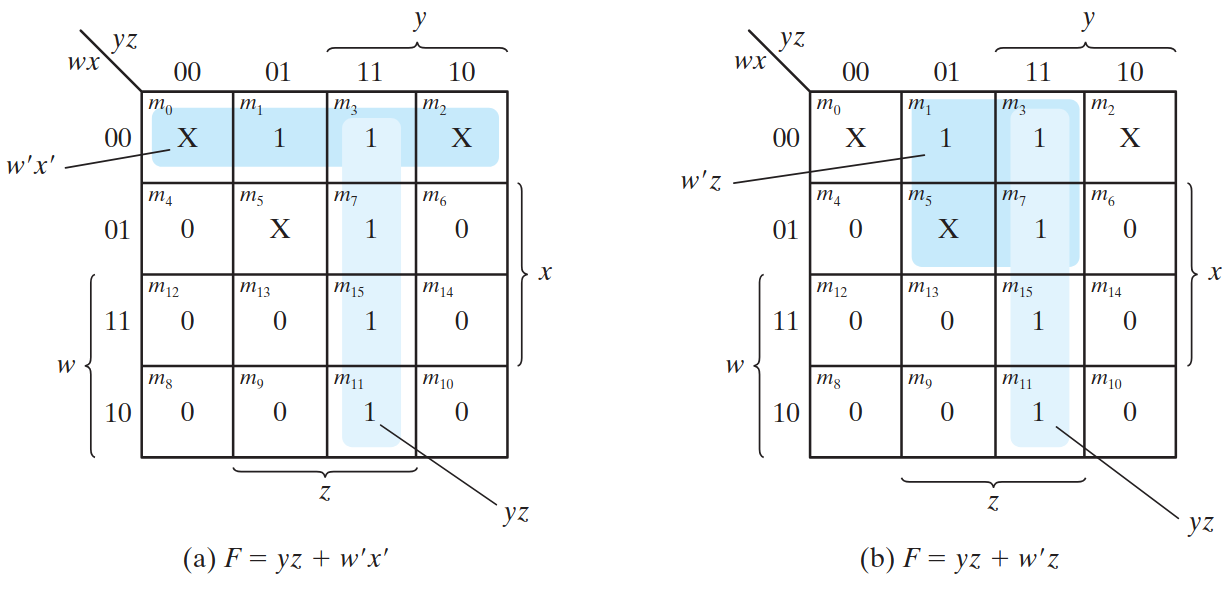
\includegraphics[width=0.9\textwidth]{figs/don.png}
    \end{center}
    \end{itemize}
\end{frame}


\section[Conclusion]{Conclusion}
\begin{frame}{Conclusion}
    \begin{itemize}
        \item Gate minimization reduces hardware cost and improves efficiency.
        \item K-Maps provide a systematic simplification method.
        \item Understanding simplification techniques aids in modern digital design.
    \end{itemize}
\end{frame}




\begin{frame}
	\transglitter<1>
	\frametitle{Once Again...}
	%\pause
	\begin{block}{ }
		\begin{center} \alert{\Huge\bf THANK YOU!} \end{center}
	\end{block}
\end{frame}



\end{document}


